
\documentclass[12pt]{book}

\usepackage{amsmath}
\usepackage{amssymb}
\usepackage{amsthm}

\usepackage{algorithm}
\usepackage{algpseudocode}

\usepackage{fancyheadings}
\usepackage{setspace}
\usepackage{color}
\usepackage{caption}
\usepackage{float}
\usepackage{fancyvrb}
\usepackage{graphicx}
\usepackage{listings}
\usepackage{float}
\usepackage{titlesec}
\usepackage{fancyhdr}
\usepackage{lipsum}
\usepackage{imakeidx}
\usepackage[bookmarksnumbered=true,colorlinks=true,linkcolor=blue]{hyperref}

\textwidth=17cm
\textheight=22.5cm

\setlength{\oddsidemargin}{-0.1in}
\setlength{\evensidemargin}{-0.1in}

\topmargin=3pt
\abovecaptionskip=3pt
\belowcaptionskip=3pt


\marginparwidth 0pt \marginparsep 10pt
\columnsep 0.5in \parindent  18pt   \parskip  0pt
\setlength{\itemsep}{.5pt}
\setlength{\parsep}{0pt}
\setlength\parindent{0pt}
\setcounter{secnumdepth}{4}

\definecolor{verbgray}{gray}{0.9}

\lstnewenvironment{evb}{%
      \lstset{backgroundcolor=\color{verbgray},
        frame=single, framerule=0pt, basicstyle=\footnotesize\ttfamily,
              columns=fullflexible, keepspaces=true, belowskip=0.3cm}}{}

\definecolor{shadecolor}{rgb}{.9, .9, .9}

%%%%%% nverb
\lstset{
        basicstyle=\color{blue} \ttfamily,
}
\lstdefinestyle{inline}{
    columns=fullflexible,breaklines=true
}
\newcommand{\nverb}[1]{\lstinline[style=inline]!#1!}

\pagestyle{fancy}

\fancyhead[RE]{\leftmark}
\fancyhead[LO]{\rightmark}
\fancyhead[LE,RO]{}
\renewcommand\sectionmark[1]{\markright{\thesection.\ #1}}

\newcommand{\namelistlabel}[1]{\mbox{#1}\hfill}
\newenvironment{namelist}[1]{%
\begin{list}{}
  {\let\makelabel\namelistlabel
  \settowidth{\labelwidth}{#1}
  \setlength{\leftmargin}{1.1\labelwidth}}
  }{%
\end{list}}

\makeindex

\begin{document}

\begin{titlepage}
\begin{center}

\vspace{5cm}
\begin{spacing}{2.5}
\vspace{5cm}
\textbf{} \\[1.5cm]
\textbf{\Huge SXAMG: a Serial Algebraic Multigrid Solver Library} \\[0.5cm]
\textbf{VERSION 1.0}
\vspace*{\fill}
\end{spacing}

\begin{spacing}{1.15}
\textnormal{\large Hui Liu}
\end{spacing}
\end{center}
\end{titlepage}

\tableofcontents

\setlength{\parskip}{8pt}

\clearpage
\pagenumbering{arabic}


\chapter{Introduction}

%%%%%%%%%%%%%%%%%%%%%%%%%%%%%%%%%%%%%%%%%%%%%%%%%%%%%%%%%%%%%%%%%%%%%
\section{Overview}

\verb|SXAMG| is an AMG (Algebraic Multi-Grid) solver 
library for sparse linear system, \verb|Ax = b|. 
The initial code is from FASP project, \url{http://fasp.sourceforge.net}, which implements a collection of Krylov solvers, AMG solvers and preconditioners.

The library is serial and written by C.
It is designed for Linux, Unix and Mac systems. However, 
it is also possible to compile under Windows if user generates a file \verb|include/config.h| manually,
where \verb|USE_UNIX| should be set to 0. 

\verb|SXAMG| rewrites all the data structures, subroutines, and file structures, and it removes many components of the original implementation and third-party package dependency.
The purpose of this refactorization is to provide a standalone AMG solver to support 
other numerical applications and to validate new ideas in the future. 
The \verb|SXAMG| can serve as a solver and a preconditioning method.

%%%%%%%%%%%%%%%%%%%%%%%%%%%%%%%%%%%%%%%%%%%%%%%%%%%%%%%%%%%%%%%%%%%%%
\section{License}

The package uses General Public License (GPL) license. 
If you have any issue, please contact the developer: \href{mailto: hui.sc.liu@gmail.com}{hui.sc.liu@gmail.com}

%%%%%%%%%%%%%%%%%%%%%%%%%%%%%%%%%%%%%%%%%%%%%%%%%%%%%%%%%%%%%%%%%%%%%
\section{Citation}

If you use this library for your research, proper citation will be appreciated.
The \verb|SXAMG| library can be cited as,
\begin{evb}
@misc{sxamg-library,
    author="Hui Liu",
    title="SXAMG: a Serial Algebraic Multigrid Solver Library",
    year="2017",
    note={\url{https://github.com/huiscliu/sxamg/}}
}
\end{evb}


%%%%%%%%%%%%%%%%%%%%%%%%%%%%%%%%%%%%%%%%%%%%%%%%%%%%%%%%%%%%%%%%%%%%%
\section{Website}
The official website for \verb|SXAMG| is \url{https://github.com/huiscliu/sxamg/}.



\chapter{Installation}


\verb|SXAMG| uses {\color{blue}{\nverb{autoconf}}} and {\color{blue}{\nverb{make}}} 
to detect system parameters, to build and to install.

\section{Configuration}
The simplest way to configure is to run command:
\begin{evb}
./configure
\end{evb}

This command will try to find optional packages if applicable and set system parameters.

\section{Options}
The script {\color{blue}{configure}} has many options, if user would like to check, 
run command:
\begin{evb}
./configure --help
\end{evb}

Output will be like this,
\begin{evb}
`configure' configures this package to adapt to many kinds of systems.

Usage: ./configure [OPTION]... [VAR=VALUE]...

To assign environment variables (e.g., CC, CFLAGS...), specify them as
VAR=VALUE.  See below for descriptions of some of the useful variables.

....

Optional Features:
  --disable-option-checking  ignore unrecognized --enable/--with options
  --disable-FEATURE       do not include FEATURE (same as --enable-FEATURE=no)
  --enable-FEATURE[=ARG]  include FEATURE [ARG=yes]
  --enable-rpath          enable use of rpath (default)
  --disable-rpath         disable use of rpath
  --with-rpath-flag=FLAG  compiler flag for rpath (e.g., "-Wl,-rpath,")
  --disable-assert        turn off assertions
  --enable-big-int        use long int for INT
  --disable-big-int       use int for INT (default),
  --with-int=type         integer type(long|long long)
  --enable-long-double    use long double for FLOAT
  --disable-long-double   use double for FLOAT (default)

Some influential environment variables:
  CC          C compiler command
  CFLAGS      C compiler flags
  LDFLAGS     linker flags, e.g. -L<lib dir> if you have libraries in a
              nonstandard directory <lib dir>
  LIBS        libraries to pass to the linker, e.g. -l<library>
  CPPFLAGS    (Objective) C/C++ preprocessor flags, e.g. -I<include dir> if
              you have headers in a nonstandard directory <include dir>
  CXX         C++ compiler command
  CXXFLAGS    C++ compiler flags
  FC          Fortran compiler command
  FCFLAGS     Fortran compiler flags
  CPP         C preprocessor
  CXXCPP      C++ preprocessor
\end{evb}

The most important options are,
\begin{itemize}
    \item \nverb{--prefix=PATH} where to install the library, and default directory is \verb|/usr/local/sxamg/|;

    \item \nverb{--enable-rpath} and \nverb{--disable-rpath}, use rpath or not, and it is enabled by default;

    \item \nverb{--enable-big-int} and \nverb{--disable-big-int}, use big integer or not, and use \nverb{int} by default;

    \item \nverb{--with-int=type}, type is \nverb{long} or \nverb{long long}. This option is checked when big integer
        is enabled (\nverb{--enable-big-int});

    \item \nverb{--enable-long-double} and \nverb{--disable-long-double}, use \nverb{long double} or not, and
        \nverb{double} is used by default;

\end{itemize}

\section{Compilation}
After configuration, \nverb{Makefile} and related scripts will be set correctly.
A simple {\color{blue}\textbf{make}} command can compile the package,

\begin{evb}
make
\end{evb}

\section{Installation}
Run command:
\begin{evb}
make install
\end{evb}
The package will be installed to a directory. The default is \nverb{/usr/local/sxamg/}. 
A different directory can be set by \nverb{--prefix=DIR} when configuring, 
such as \nverb{--prefix=/usr/sxamg/}.



\chapter{Basics}

This chapter introduces basic types, matrix and vector management.

\section{Data Types}

\verb|SXAMG| has two data types, \verb|SX_FLOAT| and \verb|SX_INT|, for floating-point number
and integer, respectively. They are defined as:
\begin{evb}
#if USE_LONG_DOUBLE
typedef long double              SX_FLOAT;
#else
typedef double                   SX_FLOAT;
#endif

#if USE_LONG_LONG
typedef signed long long int     SX_INT;
#elif USE_LONG
typedef signed long int          SX_INT;
#else
typedef signed int               SX_INT;
#endif

\end{evb}

The macros, \nverb{USE_LONG_DOUBLE}, \nverb{USE_LONG_LONG} and \nverb{USE_LONG}, are set by \nverb{configure} to
control the real types, such as \nverb{long int} and \nverb{long double}. 
User can control through  \nverb{configure} options.

\section{Matrix}
\nverb{SX_MAT} defines a CSR matrix. The index is from \nverb{0} (zero) following C convention. 
The meanings of the members are the same as usual.
\begin{evb}
typedef struct SX_MAT
{
    SX_INT num_rows;   /* number of rows */
    SX_INT num_cols;   /* number of columns */
    SX_INT num_nnzs;   /* number of non-zeros (entries) */

    SX_INT   *Ap;      /* offset of each row */
    SX_INT   *Aj;      /* column indices */
    SX_FLOAT *Ax;      /* values */

} SX_MAT;
\end{evb}

\subsection{Matrix Management}

\subsubsection{Create}

\nverb{sx_mat_struct_create} creates the structure of a matrix. The memory is allocated
but no value is set.
\begin{evb}
SX_MAT sx_mat_struct_create(const SX_INT nrow, const SX_INT ncol, const SX_INT nnz);
\end{evb}

\nverb{sx_mat_create} creates a CSR matrix by user input. This function allocates memory
and copies values to the matrix.
\begin{evb}
SX_MAT sx_mat_create(SX_INT nrow, SX_INT ncol, SX_INT *Ap, SX_INT *Aj, SX_FLOAT *Ax);
\end{evb}

\subsubsection{Destroy}
\nverb{sx_mat_destroy} destroys a matrix and frees its memory.
\begin{evb}
void sx_mat_destroy(SX_MAT *A);
\end{evb}

\subsubsection{Transpose}
\nverb{sx_mat_trans} gets transpose of a matrix.
\begin{evb}
SX_MAT sx_mat_trans(SX_MAT *A);
\end{evb}

\subsubsection{Sort}
\nverb{sx_mat_sort} sorts column indices in ascending manner.
\begin{evb}
void sx_mat_sort(SX_MAT *A);
\end{evb}

\section{Vector}

\nverb{SX_VEC} defines floating-point vector. {\color{blue} $n$} is the length of the vector, and 
{\color{blue} $d$} stores the values.
\begin{evb}
typedef struct SX_VEC 
{
    SX_INT   n;
    SX_FLOAT *d;

} SX_VEC;
\end{evb}

\subsection{Vector Management}

\subsubsection{Create}
\nverb{sx_vec_create} creates a vector of length $m (m \ge 0)$.
\begin{evb}
SX_VEC sx_vec_create(SX_INT m);
\end{evb}

\subsubsection{Destroy}

\nverb{sx_vec_destroy} destroys a vector and frees its memory.
\begin{evb}
void sx_vec_destroy(SX_VEC *u);
\end{evb}

\subsubsection{Set Value}

\nverb{sx_vec_set_value} sets equal value to each component.
\begin{evb}
void sx_vec_set_value(SX_VEC *x, SX_FLOAT val);
\end{evb}

\nverb{sx_vec_set_entry} sets value: $x[i] = val$.
\begin{evb}
void sx_vec_set_entry(SX_VEC *x, SX_INT i, SX_FLOAT val);
\end{evb}

\subsubsection{Get Value}
\nverb{sx_vec_get_entry} returns value of $x[i]$.
\begin{evb}
SX_FLOAT sx_vec_get_entry(const SX_VEC *x, SX_INT i);
\end{evb}

\subsubsection{Copy}
\nverb{sx_vec_cp} copies values from source vector and to destination vector, and the two vectors
should have the same length.
\begin{evb}
void sx_vec_cp(const SX_VEC *src, SX_VEC *des);
\end{evb}

\section{BLAS Operations}
Some level 1 and level 2 BLAS operations are implemented for internal use.

\subsection{Vector}
\nverb{sx_blas_vec_norm2} calculates L2 norm.
\begin{evb}
SX_FLOAT sx_blas_vec_norm2(const SX_VEC *x);
\end{evb}

\nverb{sx_blas_vec_dot} calculates dot product.
\begin{evb}
SX_FLOAT sx_blas_vec_dot(const SX_VEC *x, const SX_VEC *y);
\end{evb}

\nverb{sx_blas_vec_axpyz} computes: $z = a * x + y$.
\begin{evb}
void sx_blas_vec_axpyz(SX_FLOAT a, const SX_VEC *x, const SX_VEC *y, SX_VEC *z);
\end{evb}

\nverb{sx_blas_vec_axpyz} computes: $z = a * x + b * y$.
\begin{evb}
void sx_blas_vec_axpyz(SX_FLOAT a, const SX_VEC *x, SX_FLOAT b, const SX_VEC *y, SX_VEC *z);
\end{evb}

\nverb{sx_blas_vec_axpy} computes: $y = a * x + y$.
\begin{evb}
void sx_blas_vec_axpy(SX_FLOAT a, const SX_VEC *x, SX_VEC *y);
\end{evb}

\nverb{sx_blas_vec_axpby} computes: $y = a * x + b * y$.
\begin{evb}
void sx_blas_vec_axpy(SX_FLOAT a, const SX_VEC *x, SX_FLOAT b, SX_VEC *y);
\end{evb}

\subsection{Matrix-Vector}
\nverb{sx_blas_mat_amxpy} computes: $ y = y + a * A * x $.
\begin{evb}
void sx_blas_mat_amxpy(SX_FLOAT a, const SX_MAT *A, const SX_VEC *x, SX_VEC *y);
\end{evb}

\nverb{sx_blas_mat_mxy} computes: $y = A * x $.
\begin{evb}
void sx_blas_mat_mxy(const SX_MAT *A, const SX_VEC *x, SX_VEC *y);
\end{evb}

\subsection{Matrix-Matrix}
\nverb{sx_blas_mat_rap} returns the matrix-matrix product: $ R * A * P$.
\begin{evb}
SX_MAT sx_blas_mat_rap(const SX_MAT *R, const SX_MAT *A, const SX_MAT *P);
\end{evb}

\chapter{AMG Solver}

If $A$ is a positive-definite square matrix, the AMG methods
\cite{AMG, AMG-OR, Stuben2, BMR, falgout, psm} have proved to be
efficient methods and they are also scalable \cite{rsamg}.

AMG methods have hierarchical structures, which is shown in Figure \ref{fig-amg}.
A coarse grid is constructed when entering a coarser level.
To calculate a coarser matrix, a restriction operator $R_l$ and
an interpolation (prolongation) operator $P_l$ need to be determined.
In general, the restriction operator $R_l$ is the transpose of the interpolation (prolongation) operator $P_l$:

\[
R_l = P_l^T.
\]
The matrix on the coarser grid is calculated as
\begin{equation}
A_{l + 1} = R_l A_l P_l.
\end{equation}
We know that a high frequency error is easier to converge on a fine grid than a low frequency error, and
for the AMG methods,
the restriction operator, $R_l$, projects the error from a finer grid onto a coarser grid and
converts a low frequency error to a high frequency error.
The interpolation operator transfers a solution on a coarser
grid to that on a finer grid.
Its setup phase for the AMG methods on each level $l$ ($0 \leq l < L$) is formulated in
Algorithm \ref{alg-amg-setup}, where a coarser grid, an interpolation operator, a restriction
operator, a coarser matrix and post- and pre-smoothers are constructed.
By repeating the algorithm, an $L$-level system can be built.
The solution of the AMG methods is recursive and is formulated in Algorithm \ref{alg-amg-solve}, which
shows one iteration of AMG.

\begin{figure}[!htb]
    \centering
    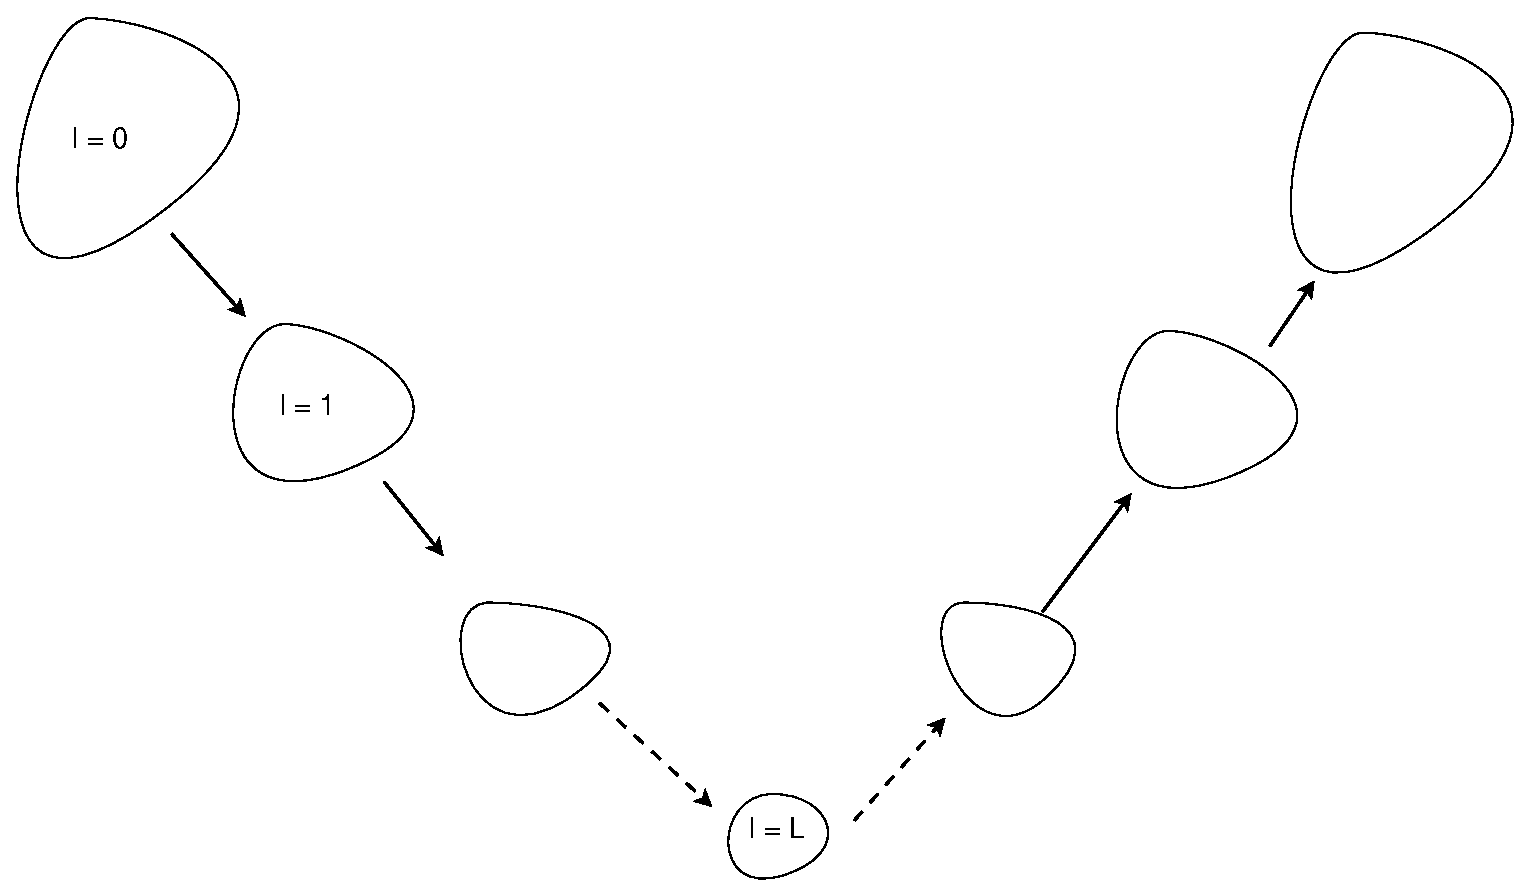
\includegraphics[width=0.650\linewidth]{amg}
    \caption{Structure of AMG solver.}
    \label{fig-amg}
\end{figure}

\begin{algorithm}[!htb]
\caption{AMG setup Algorithm} \label{alg-amg-setup}
\begin{algorithmic}[1]
  \State Calculate strength matrix $S$.
  \State Choose coarsening nodes set $\omega_{l+1}$ according to strength matrix $S$, such that $\omega_{l+1} \subset \omega_{l}$.
  \State Calculate prolongation operator $P_l$.
  \State Derive restriction operator $R_l = P_l^T$.
  \State Calculate coarse matrix $A_{l+1}$: $A_{l+1} = R_l \times A_l \times P_l$.
  \State Setup pre-smoother $S_l$ and post-smoother $T_l$.
\end{algorithmic}
\end{algorithm}

\begin{algorithm}[!htb]
\caption{AMG V-cycle Solution Algorithm: amg\_solve($l$)} \label{alg-amg-solve}
\begin{algorithmic}%[1]
\State Require: $b_l$, $x_l$, $A_l$, $R_l$, $P_l$, $S_l$, $T_l$, $0 \leq l < L$
\State
\State $b_0 = b$

\If {($l < L$)}
  \State $x_l = S_l(x_l, A_l, b_l)$
  \State $r = b_l - A_lx_l$
  \State $b_{r+1} = R_lr$
  \State amg\_solve($l+1$)
  \State $x_l = x_l + P_l x_{l+1}$
  \State $x_l = T_l(x_l, A_l, b_l)$
\Else
  \State $x_l = A_l^{-1}b_l$
\EndIf

\State x = $x_0$

\end{algorithmic}
\end{algorithm}

The Cleary-Luby-Jones-Plassman (CLJP) coarsening
algorithm was proposed by Cleary \cite{cljp1} based on the algorithms developed
by Luby \cite{cljp3} and Jones and Plassman \cite{cljp2}. The standard RS coarsening algorithm
has also been parallelized \cite{HYPRE2}. Falgout et al. developed a parallel coarsening algorithm,
the Falgout coarsening algorithm, which has been implemented in HYPRE \cite{HYPRE2}. Yang et al. proposed
HMIS and PMIS coarsening algorithms for a coarse grid selection \cite{pmis}. Various parallel smoothers
and interpolation operators have also been studied by Yang et al \cite{HYPRE2,pmis}.

\section{Data Structures}

\nverb{SX_SM_TYPE} defines smoother types. The following smoothers are implemented,
\begin{evb}
typedef enum
{
    SX_SM_JACOBI    = 1,  /**< Jacobi smoother */
    SX_SM_GS        = 2,  /**< Gauss-Seidel smoother */
    SX_SM_SGS       = 3,  /**< Symmetric Gauss-Seidel smoother */
    SX_SM_SOR       = 4,  /**< SOR smoother */
    SX_SM_SSOR      = 5,  /**< SSOR smoother */
    SX_SM_GSOR      = 6,  /**< GS + SOR smoother */
    SX_SM_SGSOR     = 7,  /**< SGS + SSOR smoother */
    SX_SM_POLY      = 8,  /**< Polynomial smoother */
    SX_SM_L1DIAG    = 9,  /**< L1 norm diagonal scaling smoother */

} SX_SM_TYPE;
\end{evb}

\nverb{SX_COARSEN_TYPE} defines coarsening types, including classical RS coarsening and
classical RS coarsening with positive off-diagonals.
\begin{evb}
typedef enum
{
    SX_COARSE_RS      = 1,  /**< Classical */
    SX_COARSE_RSP     = 2,  /**< Classical, with positive offdiags */

} SX_COARSEN_TYPE;
\end{evb}


\nverb{SX_INTERP_TYPE} defines interpolation types, including direct interpolation
and standard interpolation.
\begin{evb}
typedef enum
{
    SX_INTERP_DIR     = 1,  /**< Direct interpolation */
    SX_INTERP_STD     = 2,  /**< Standard interpolation */

} SX_INTERP_TYPE;
\end{evb}


\nverb{SX_AMG_PARS} defines AMG parameters. The meaning of each member is explained as comment. For example,
\nverb{cycle_itr}
determines the cycle type: 1 for V-cycle, 2 for W-cycle..
\begin{evb}
typedef struct SX_AMG_PARS
{
    SX_INT verb;

    SX_INT cycle_itr;          /** type of AMG cycle, 1 is for V, W if greater than 1 */
    SX_FLT tol;                /** stopping tolerance for AMG solver */
    SX_FLT ctol;               /** stopping tolerance for coarsest solver */
    SX_INT maxit;              /** maximal number of iterations of AMG */

    SX_COARSEN_TYPE cs_type;     /** coarsening type */
    SX_INT max_levels;           /** max number of levels of AMG */
    SX_INT coarse_dof;           /** max number of coarsest level DOF */

    SX_SM_TYPE smoother;         /** smoother type */
    SX_FLT     relax;            /** relax parseter for SOR smoother */
    SX_INT     cf_order;         /** False (0): nature order, True (1): C/F order */
    SX_INT     pre_iter;         /** number of presmoothers */
    SX_INT     post_iter;        /** number of postsmoothers */
    SX_INT     poly_deg;         /** degree of the polynomial smoother */

    SX_INTERP_TYPE interp_type;  /** interpolation type */
    SX_FLT strong_threshold;     /** strong connection threshold for coarsening */
    SX_FLT max_row_sum;          /** maximal row sum parseter */
    SX_FLT trunc_threshold;      /** truncation threshold */

} SX_AMG_PARS;
\end{evb}

\nverb{SX_RTN} is for return values.
\begin{evb}
typedef struct SX_RTN
{
    SX_FLT ares;     /* absolute residual */
    SX_FLT rres;     /* relative residual */
    SX_INT nits;     /* number of iterations */

} SX_RTN;
\end{evb}

\section{Management}

\subsection{Initialize Parameters}

\nverb{sx_amg_pars_init} sets default parameters.
\begin{evb}
void sx_amg_pars_init(SX_AMG_PARS *pars);
\end{evb}

\subsection{Setup}
\nverb{sx_amg_setup} setups the hierarchical struture of AMG solver using given parameters.
\begin{evb}
void sx_amg_setup(SX_AMG *mg, SX_MAT *A, SX_AMG_PARS *pars);
\end{evb}

\subsection{Solve}

\nverb{sx_solver_amg_solve} solves the linear system using AMG method. The AMG object has to be
set up before using, the \nverb{x} has initial value and \nverb{b} is the right-hand side.
\begin{evb}
SX_RTN sx_solver_amg_solve(SX_AMG *mg, SX_VEC *x, SX_VEC *b);
\end{evb}

\nverb{sx_solver_amg} solves the linear system using AMG method. This function is a high level 
interface, and user can call it to solve a linear system, which will setup the AMG object,
solve and destroy the AMG object. If \nverb{pars} is \verb|NULL|, then default parameters
will be applied.
\begin{evb}
SX_RTN sx_solver_amg(SX_MAT *A, SX_VEC *x, SX_VEC *b, SX_AMG_PARS *pars);
\end{evb}

\subsection{Destroy}
\nverb{sx_amg_data_destroy} destroys the AMG object.
\begin{evb}
void sx_amg_data_destroy(SX_AMG *mg);
\end{evb}


\chapter{Utilities}

\section{Print}

\nverb{sx_set_log} sets log file. If log file is set, all screen prints will be stored to log file,
\begin{evb}
void sx_set_log(FILE *io);
\end{evb}

\nverb{sx_printf} prints info to screen, if log file is set, it prints to log file and screen,
\begin{evb}
int sx_printf(const char *fmt, ...);
\end{evb}

\section{Memory}

\nverb{sx_mem_malloc} allocates memory,
\begin{evb}
void * sx_mem_malloc(size_t size);
\end{evb}

\nverb{sx_mem_calloc} allocates and initializes memory,
\begin{evb}
void * sx_mem_calloc(size_t size, SX_INT type);
\end{evb}

\nverb{sx_mem_realloc} reallocates memory,
\begin{evb}
void * sx_mem_realloc(void *oldmem, size_t tsize);
\end{evb}

\nverb{sx_mem_free} frees memory,
\begin{evb}
void sx_mem_free(void *mem);
\end{evb}

\section{Performance}

\nverb{sx_gettime} returns current time stamp, if \nverb{t} is not \nverb{NULL}, 
result will be written to \nverb{t},
\begin{evb}
SX_FLOAT sx_gettime(SX_FLOAT *t);
\end{evb}

\chapter{How to Use}

\section{Solver}

This example shows how to use SXAMG as a solver.  Five steps are required to call: 
\begin{enumerate}
    \item \nverb{sx_amg_pars_init} initializes default AMG parameters, 
        and user can check their value from source code;

    \item Re-define parameters. This step is optional.

    \item Input matrix, initial guess and right-hand side should be constructed.

    \item \nverb{sx_solver_amg} setups, solves and destroys the AMG system, 
        and the solution is stored by \nverb{x}.

    \item Free memories.

\end{enumerate}

\begin{evb}
{
    SX_AMG_PARS pars;
    SX_MAT A;
    SX_VEC b, x;
    int verb = 2;
    SX_RTN rtn;
    
    /* step 1: default pars */
    sx_amg_pars_init(&pars);

    /* step 2: redefine parameters */
    pars.maxit = 1000;
    pars.verb = 2;
    
    /* step 3: set A, b, initial x */
    ....
    
    /* step 4: solve the system */
    rtn = sx_solver_amg(&A, &x, &b, &pars);
    
    /* step 5: free memory */
    sx_mat_destroy(&A);
    sx_vec_destroy(&b);
    sx_vec_destroy(&x);
}
\end{evb}


\section{Lower Level Interface}

Sometimes user needs to store the AMG object and re-uses it, such as preconditioner.
This example exposes more details of the AMG solver, where seven steps are required:
\begin{enumerate}
    \item initialize default parameters;

    \item re-define parameters if default parameters do not meet requirement;

    \item setup input matrix \nverb{A}, which is a standard CSR matrix;

    \item setup AMG object;

    \item setup initial guess and right-hand side;

    \item solve the linear system using given \nverb{x} and \nverb{b};

    \item free memories;

\end{enumerate}

Here user can call step 1) to 4) once in the beginning stage, call 5) and 6) as many as required, 
and call step 7) in the end stage of the program.

\begin{evb}
{
    SX_AMG_PARS pars;
    SX_MAT A;
    SX_VEC b, x;
    int verb = 2;
    SX_AMG *mg;
    SX_RTN rtn;
    
    /* step 1: pars */
    sx_amg_pars_init(&pars);

    /* step 2: re-define parameters */
    pars.maxit = 1000;
    pars.verb = 2;
    
    /* step 3: input A */
    ....

    /* Step 4: setup AMG setup object */
    mg = sx_amg_setup(&A, &pars);

    /* Step 5: setup rhs and initial guess */
    x = sx_vec_create(A.num_rows);
    sx_vec_set_value(&x, 1.0);

    b = sx_vec_create(A.num_rows);
    sx_vec_set_value(&b, 1.0);

    /* step 6: solve */
    rtn = sx_solver_amg_solve(mg, &x, &b);

    /* step 7: free memories */
    sx_mat_destroy(&A);
    sx_vec_destroy(&b);
    sx_vec_destroy(&x);
    sx_amg_data_destroy(&mg);
}
\end{evb}




\backmatter

\begin{thebibliography}{00}
\bibitem{Stuben2}
{JW Ruge and K St\"{u}ben}, {Algebraic multigrid (AMG)},
in: S.F. McCormick (Ed.), Multigrid Methods, Frontiers in Applied Mathematics, Vol. 5, SIAM, Philadelphia, 1986.

\bibitem{BMR}
{A Brandt, SF McCormick, J Ruge},
Algebraic multigrid (AMG) for sparse matrix equations
D.J. Evans (Ed.), Sparsity and its Applications, Cambridge University Press, Cambridge, 1984, 257--284.

\bibitem{falgout}
RD Falgout, An Introduction to Algebraic Multigrid, Computing in Science and Engineering,
Special Issue on Multigrid Computing, 8, 2006, 24--33.

\bibitem{AMG-OR}
K. St\"{u}ben, T. Clees, H. Klie, B. Lou, M.F. Wheeler,
Algebraic multigrid methods (AMG) for the efficient solution of fully implicit formulations in reservoir simulation,
SPE Reservoir Simulation Symposium. 2007.

\bibitem{AMG}
K. St\"{u}ben,
A review of algebraic multigrid,
Journal of Computational and Applied Mathematics 128.1 (2001): 281-309.

\bibitem{psm}
UM Yang, On the Use of Relaxation Parameters in Hybrid Smoothers,
Numerical Linear Algebra With Applications, 11, (2004), 155-172.

\bibitem{rsamg}
{AJ Cleary, RD Falgout, VE Henson, JE Jones, TA Manteuffel, SF McCormick,
GN Miranda, JW Ruge}, {Robustness and Scalability of Algebraic Multigrid}, SIAM J. Sci. Comput., 21, 2000, 1886--1908.

\bibitem{HYPRE2}
R. D. Falgout, and U.M. Yang, HYPRE: A library of high performance preconditioners,
Lecture Notes in Computer Science, Springer Berlin Heidelberg, 2002. 632-641.

\bibitem{cljp1}
AJ Cleary, RD Falgout, VE Henson, JE Jones, Coarse grid selection for parallel algebraic multigrid, in Proceedings of the
fifth international symposium on solving irregularly structured problems in parallel, Springer-Verlag, New York, 1998.

\bibitem{cljp2}
MT Jones, PE Plassman, A parallel graph coloring heuristic, SIAM Journal on Scientific Computing, 14(1993): 654-669.

\bibitem{cljp3}
M Luby, A simple parallel algorithm for the maximal independent set problem,
SIAM Journal on Computing, 15(1986), 1036-1053.

\bibitem{pmis}
Hans~DS, Yang~UM, Heys~J,
Reducing Complexity in Parallel Algebraic Multigrid Preconditioners,
SIAM Journal on Matrix Analysis and Applications 27, (2006), 1019-1039.
\end{thebibliography}

\end{document}
